\documentclass[runningheads]{llncs}

\usepackage[T1]{fontenc}
\usepackage{lmodern}
\usepackage{amssymb,amsmath}
\usepackage{ifxetex,ifluatex}
\usepackage{fixltx2e} % provides \textsubscript
\usepackage{float}
\usepackage[labelfont=bf]{caption}
\usepackage{subfig}
\emergencystretch=1em
% use upquote if available, for straight quotes in verbatim environments

%\let\origfigure=\figure
%\let\endorigfigure=\endfigure
%\renewenvironment{figure}[1][]{%
	 %\origfigure[H]
%}{%
	 %\endorigfigure
%}

\captionsetup[figure]{labelfont={bf},name={Fig.},labelsep=period}

% lncs 
\usepackage{makeidx}
\institute{\textsuperscript{1} Department of Computer Science and
Engineering, SRM Institute of Science and Technology, Vadapalani Campus,
Chennai - 26, \\ \texttt{\{vishalbalaji,arunnehru.aucse\}@gmail.com}}

\makeatletter
\let\oldsubsubsection\subsubsection
\renewcommand\subsubsection{\@ifstar{\oldsubsubsection}{\oldsubsubsection*}}
\makeatother

\makeatletter
\let\oldparagraph\paragraph
\renewcommand\paragraph{\@ifstar{\oldparagraph}{\oldparagraph*}}
\makeatother

\IfFileExists{upquote.sty}{\usepackage{upquote}}{}
\ifnum 0\ifxetex 1\fi\ifluatex 1\fi=0 % if pdftex
  \usepackage[utf8]{inputenc}
\else % if luatex or xelatex
  \ifxetex
    \usepackage{mathspec}
    \usepackage{xltxtra,xunicode}
  \else
    \usepackage{fontspec}
  \fi
  \defaultfontfeatures{Mapping=tex-text,Scale=MatchLowercase}
  \newcommand{\euro}{€}
\fi
% use microtype if available
\IfFileExists{microtype.sty}{\usepackage{microtype}}{}
\usepackage{longtable,booktabs}
\usepackage{graphicx}
% Redefine \includegraphics so that, unless explicit options are
% given, the image width will not exceed the width of the page.
% Images get their normal width if they fit onto the page, but
% are scaled down if they would overflow the margins.
\makeatletter
\def\ScaleIfNeeded{%
  \ifdim\Gin@nat@width>\linewidth
    \linewidth
  \else
    \Gin@nat@width
  \fi
}
\makeatother
\let\Oldincludegraphics\includegraphics
{%
 \catcode`\@=11\relax%
 \gdef\includegraphics{\@ifnextchar[{\Oldincludegraphics}{\Oldincludegraphics[width=\ScaleIfNeeded]}}%
}%
\ifxetex
  \usepackage[setpagesize=false, % page size defined by xetex
              unicode=false, % unicode breaks when used with xetex
              xetex]{hyperref}
\else
  \usepackage[unicode=true]{hyperref}
\fi
\hypersetup{breaklinks=true,
            bookmarks=true,
            pdfauthor={},
            pdftitle={Predictive Analysis of Employee Promotion},
            colorlinks=true,
            citecolor=blue,
            urlcolor=blue,
            linkcolor=blue,
            pdfborder={0 0 0}}
\urlstyle{same}  % don't use monospace font for urls
\setlength{\parindent}{0pt}
\setlength{\parskip}{6pt plus 2pt minus 1pt}
\setlength{\emergencystretch}{3em}  % prevent overfull lines
\setcounter{secnumdepth}{5}

\title{Predictive Analysis of Employee Promotion}
\author{Vishal Balaji D\inst{1}\orcidID{0000-1111-2222-3333} and J.
Arunnehru\inst{1}\orcidID{1111-2222-3333-4444}}
\date{}
\makeatletter
\@ifpackageloaded{subfig}{}{\usepackage{subfig}}
\@ifpackageloaded{caption}{}{\usepackage{caption}}
\captionsetup[subfloat]{margin=0.5em}
\AtBeginDocument{%
\renewcommand*\figurename{Figure}
\renewcommand*\tablename{Table}
}
\AtBeginDocument{%
\renewcommand*\listfigurename{List of Figures}
\renewcommand*\listtablename{List of Tables}
}
\@ifpackageloaded{float}{}{\usepackage{float}}
\floatstyle{ruled}
\@ifundefined{c@chapter}{\newfloat{codelisting}{h}{lop}}{\newfloat{codelisting}{h}{lop}[chapter]}
\floatname{codelisting}{Listing}
\newcommand*\listoflistings{\listof{codelisting}{List of Listings}}
\makeatother

\authorrunning{Vishal Balaji D and J. Arunnehru}

\providecommand{\tightlist}{%
  \setlength{\itemsep}{0pt}\setlength{\parskip}{0pt}}

\begin{document}
\maketitle
\begin{abstract}
The size of companies has seen an exponential growth over the years.
Corporations recruit anywhere from a few hundred to a few thousand
employees every year. With such rates, Human Resource Management in
companies is proving to be more and more significant every day. Done
manually, HRM is a laborious task, given the sheer quantity of
employees. Luckily, over the years, data analytics in HR is emerging as
an integral part in corporate operation. Yet, there remain a few tasks
that involve human involvement, one of them being selecting candidates
that are eligible for a promotion. This paper proposes a solution using
decision-tree based Machine Learning algorithms to learn from past
employee records to aid this decision making process. It explores the
usage of two Machine Learning algorithms, Random Forest and XGBoost to
predict whether an employee is eligible to receive a promotion or not
and determine what factors are responsible for that prediction.

% lncs keyword extension 
\keywords{Human Resource Management, Machine Learning, Random Forest,
XGBoost}

\end{abstract}

\hypertarget{introduction}{%
\section{Introduction}\label{introduction}}

HR analytics(see \cite{ref-Quddus2019}{1}) in
corporations plays a major role in restructuring the operand of their HR
department. A company of sizeable proportions deals with hundreds of
employee records every day. Although HR analytics has been in operation
in companies for years, some of these operations are still done
manually. Automating such processes will aid in saving valuable time and
increasing overall efficiency in the operation of the company.
Eligibility for promotions depends on numerous criteria. These criteria
vary between companies and even between departments within a company.
Currently, there is no way to automate the process of determining why
one employee should be promoted over the other, since such decisions
require logical reasoning and understanding the current environmental
factors that computers are just not capable of.

Machine Learning has been used to solve similar problems in different
domains for several years now. In areas where some kind of human
intervention is necessary, a well trained machine learning algorithm has
been proven to be an acceptable substitute, if not an ideal solution.
Here, we will be using machine learning techniques to not only predict
the promotion status of future employees, but to also determine which of
the provided attributes from the employees' data is most relevant to
making this prediction. In this paper, we explore the application the
two different machine learning algorithms, namely Random Forest(see
\cite{ref-Breiman2001}{2}) and XGBoost(see
\cite{ref-ChenG16}{3}) algorithms, to analyze a
publicly available HR dataset and determine what factors help elevate an
employee's chances of getting promoted.

In this paper, we have classified the HRM data to predict whether an
employee is a viable for a promotion. The data required for this purpose
was collected by an anonymous organization and made available to the
public through \href{https://www.kaggle.com}{Kaggle}. This dataset
consists of various differentiating features for previous candidates who
were shortlisted for a promotion and whether or not they were promoted.
This dataset consists of 14 different attributes or columns, with 54,808
total observations or rows. A comprehensive summary of the dataset is as
follows:

\begin{itemize}
\tightlist
\item
  \textbf{employee\_id(int)}: Unique id of the employee.
\item
  \textbf{department(string)}: The department to which the employee
  belongs to. Possible values are: \emph{Analytics}, \emph{Finance} ,
  \emph{HR} , \emph{Legal} , \emph{Operations}, \emph{Procurement},
  \emph{R\&D}, \emph{Sales \& Marketing}, \emph{Technology}.
\item
  \textbf{region(string)}: Region of employment. Possible values are:
  \emph{region\_10}, \emph{region\_11}, \emph{region\_12},
  \emph{region\_13}, \emph{region\_14}, \emph{region\_15},
  \emph{region\_16}, \emph{region\_17}, \emph{region\_18},
  \emph{region\_19}, \emph{region\_2}, \emph{region\_20},
  \emph{region\_21}, \emph{region\_22}, \emph{region\_23},
  \emph{region\_24}, \emph{region\_25}, \emph{region\_26},
  \emph{region\_27}, \emph{region\_28}, \emph{region\_29},
  \emph{region\_3}, \emph{region\_30}, \emph{region\_31},
  \emph{region\_32}, \emph{region\_33}, \emph{region\_34},
  \emph{region\_4}, \emph{region\_5}, \emph{region\_6},
  \emph{region\_7}, \emph{region\_8}, \emph{region\_9}.
\item
  \textbf{education(string)}: Describes the level of education of the
  employee. Possible values are: \emph{Bachelor*s}, \emph{Below
  Secondary}, \emph{Master*s \& above}.
\item
  \textbf{gender(string)}: Gender of the employee. Possible values are:
  \emph{f}, \emph{m}.
\item
  \textbf{recruitment\_channel(string)}: Channel of recruitment of the
  employee. Possible values are: \emph{referred}, \emph{sourcing},
  \emph{other}.
\item
  \textbf{no\_of trainings(int)}: Describes the number of training
  programs completed by the employee. Range: from \emph{1} to \emph{10}.
\item
  \textbf{age(int)}: Describes the age of the employee.
  previous\_year\_rating (int): Employee rating from previous year.
  Range from \emph{1} to \emph{5}.
\item
  \textbf{length\_of\_service(int)}: The service length of the employee
  in years.
\item
  \textbf{KPIs\_met \textgreater80\%(int)}: Describes whether the
  employee's \emph{Key Performance Indicators} score are greater than
  80\%. Value is \emph{1} if yes, else \emph{0}.
\item
  \textbf{awards\_won?(int)}: Whether the employee won any awards last
  year. Value is \emph{1} if yes, else \emph{0}.
\item
  \textbf{avg\_training\_score(int)}: Employee's average training score
  in training evaluations.
\item
  \textbf{is\_promoted(int)}: Whether the employee was promoted or not.
  Value is \emph{1} if yes, else \emph{0}.
\end{itemize}

The remainder of the research paper is organized as follows: A
literature review documenting past approaches and research similar to
that in this paper is represented in Section
\protect\hyperlink{literature-review}{2}. Section
\protect\hyperlink{methodology}{3} provides a detailed description of
the working dataset, outlines the preparation of the dataset and
elaborates on the two methodologies used in this paper, i.e., Random
Forest and XGBoost classifiers. In Section
\protect\hyperlink{results}{4}, we compare the outcomes of the two
methods and elaborately discuss the results. We conclude the paper in
Section \protect\hyperlink{conclusion}{5} with references and future
work.

\hypertarget{literature-review}{%
\section{Literature Review}\label{literature-review}}

A. H. Marler and J. W. Boudreau in
\cite{ref-Marler2017}{4} discuss the adoption of HR
analytics by organizations and attempts to answer some key questions
regarding its definition, inner workings, effectiveness, its impact on
corporate operation and its success factors. They conduct evidence-based
reviews of articles in peer-reviewed journals and conclude that the
available evidence is too sparse. Z. Jin et al.~in
\cite{ref-Jin2020}{5} predicts employee turnover for
companies using classification algorithms and Survival Analysis. They
employ a variation of the Random Forest algorithm named RFRSF, which
combines survival analysis for censored data processing and ensemble
learning for turnover behavior prediction. The authors contrast the
results their model with those of traditional machine learning
techniques such as Naïve Bayes, Decision Tree and Random Forest and
their algorithm predicts employee turnover with 84.65\% accuracy. J. Liu
et al.~in \cite{ref-Liu2019}{6} employ various
supervised learning approaches, utilising Logistic Regression, Random
Forest and AdaBoost algorithms. From their analysis, the Random Forest
classifier outperforms the other models, with accuracy and AUC of 85.6\%
and 88.9\% respectively along with a precision of 83.4\%.

\hypertarget{methodology}{%
\section{Methodology}\label{methodology}}

\hypertarget{feature-engineering}{%
\subsection{Feature Engineering}\label{feature-engineering}}

First off, we remove the employee\_id column as it is just a column to
distinguish records by and will not realistically impact the decision of
whether an employee is to be promoted or not. This brings down our
variable count to 13.

\hypertarget{removing-duplicate-values}{%
\subsubsection{Removing Duplicate
Values}\label{removing-duplicate-values}}

Even though we have a large volume of data, we cannot be sure that all
the observations in the dataset are unique. Looking at our data, we find
that there are 118 duplicate records that are present in our dataset.
Even though it does not seem like a significantly large number,
duplicate records will negatively impact the training process of machine
learning algorithms and may cause them to over-fit. After the removal of
the duplicate values, we have 54,690 observations left.

\hypertarget{removing-missing-values}{%
\subsubsection{Removing Missing Values}\label{removing-missing-values}}

To deal with missing values, we separate out the observations with a
NULL value for at least one variable. We also notice that only two
columns, \textbf{education} and \textbf{previous\_year\_rating} contain
null values in 2398 and 4062 observations, respectively. We rectify this
by filling in the missing attribute with the mode of that particular
attribute in all the observations where the value of the target variable
is the same as in the column with the missing value. This approach
allows us to eliminate observations with missing values while still
retaining the size of our dataset.

\hypertarget{preprocessing}{%
\subsection{Preprocessing}\label{preprocessing}}

The data is pre-processed to make it suitable for our algorithms. Since
the target variable is categorical in nature, encode its values using
one-hot encoding to optimize our models' performance. One-hot encoding
is a method of representing categorical variables in a way which can be
parsed by our machine learning models. To do so, we use the integer
representation of our target variable, where 0 corresponds to the value
\emph{no} and 1 corresponds to the value \emph{yes} and transform them
into an array of binary digits whose length is equal to the total number
of possible values(2 in our case). The digit in the array whose position
corresponds to our integer value is set to 1 while the other values are
set to 0, i.e., \emph{0} becomes \emph{{[}1, 0}, \emph{1} becomes
\emph{{[}0, 1} etc.

We also rename the values in the target column from ``0'' and ``1'' to
``no'' and ``yes'' so that the algorithm recognizes as categorical
variables. This will also aid us to make better visualizations of the
data.

\hypertarget{balancing-classes}{%
\subsection{Balancing Classes}\label{balancing-classes}}

In this dataset, there is a clear imbalance between the values of our
target variables. Out of 54,690 observations, only 4665 observations are
of class ``no,'' while 50,025 observations are of class ``yes.'' This is
a significant issue, as the difference exceeds more than 50\% of our
total data. For a machine learning algorithm to be properly able to
parse and understand the given data, there should ideally be an equal
distribution of the number of examples with the different classes that
the model is meant to classify data into. When one class takes
precedence over the other class in the dataset, the algorithm is less
likely to learn what the properties of each class are and tends to
forget the less frequent class' properties all together during training.

To ensure that this does not happen, we must make sure that there are
equal numbers of examples for both the cases. Here, we randomly sample a
subset of the data where the class is ``yes,'' as it is the class with
higher frequency and append it to the observations with the class ``no''
to generate a new, minified training set with equal number of ``yes''
and ``no'' observations. This process is called under-sampling. This
brings down the size of our dataset to 9330 observations total. Even
though it is only a fraction of the original 54,690, it is still a
significant amount and should be enough to train our algorithms along
with being balanced. The distribution of class percentage before and
after under sampling is shown fig.~\ref{fig:class_balancing}.

\begin{figure}
\centering

\subfloat[Distribution of class percentage before
under-sampling]{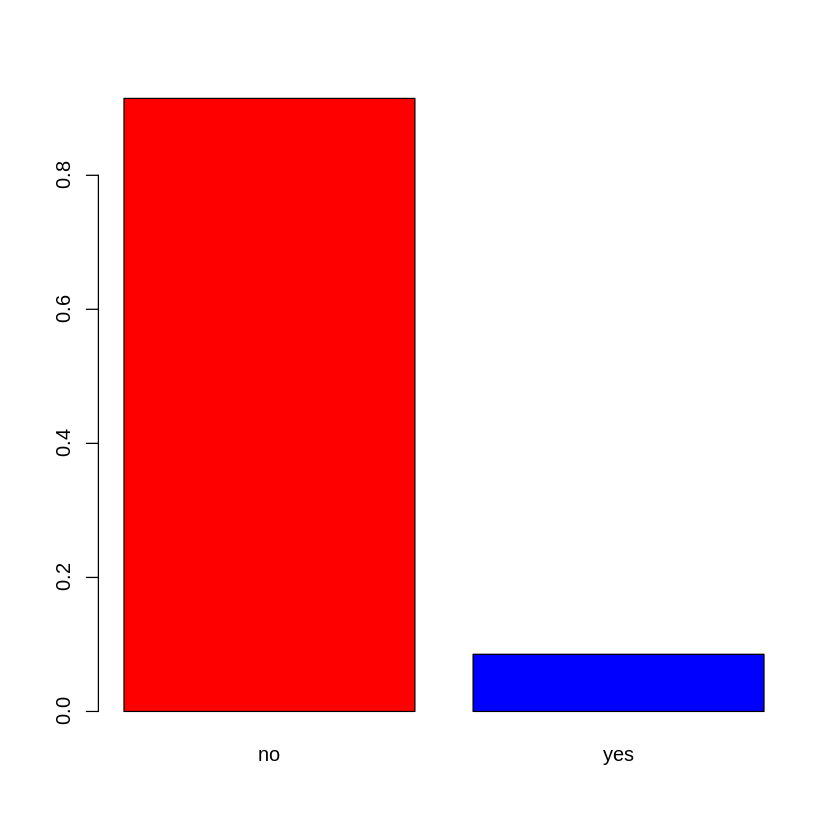
\includegraphics[width=0.49\textwidth,height=0.27\textheight]{./imgs/class_imbalance.png}}
\subfloat[Distribution of class percentage after
under-sampling]{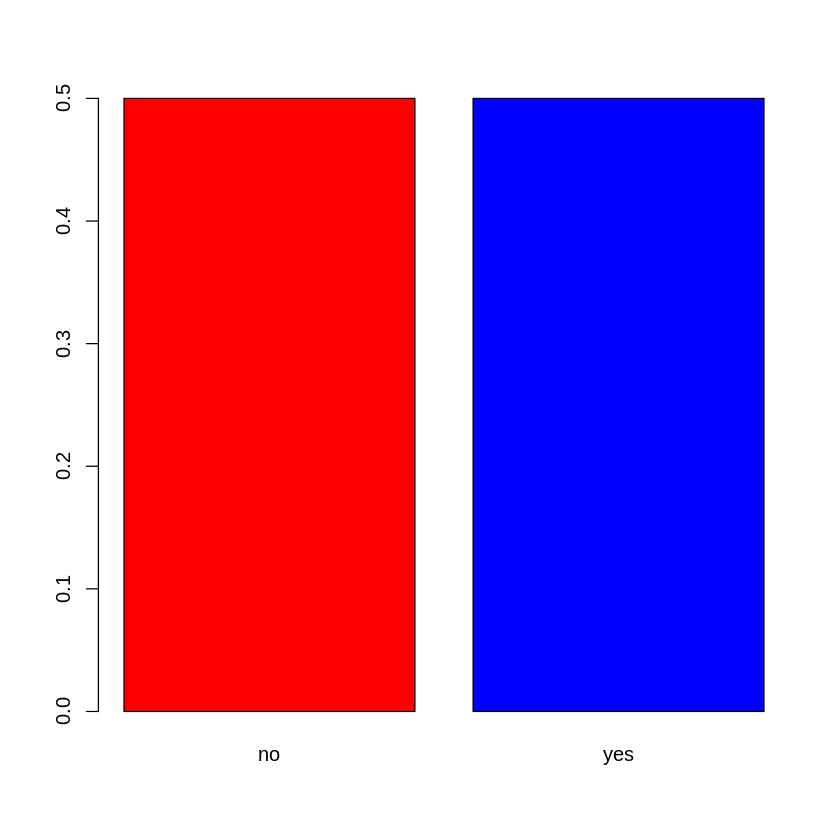
\includegraphics[width=0.49\textwidth,height=0.27\textheight]{./imgs/class_balance.png}}

\caption{Distribution of \emph{is\_promoted} class before and after
undersampling}

\label{fig:class_balancing}

\end{figure}

\hypertarget{training-and-evaluation}{%
\subsection{Training and Evaluation}\label{training-and-evaluation}}

The dataset is split into a training set and a testing set where the
testing set contains 1/5ths of the records in the dataset while the rest
belong to the training set. The resultant training and testing sets will
therefore have 7464 and 1866 observations respectively.

A Random Forest(RF) and XGBoost(XGB) model will be will be trained on
the training set and be evaluated using the K-fold cross-validation
method for the testing set. In this case, the value of K is taken to be
5. Confusion matrices will be generated for both models, which will help
us determine the accuracy with which the models classify observations as
\emph{yes} or \emph{no}.

\hypertarget{random-forest}{%
\subsubsection{Random Forest}\label{random-forest}}

The Random Forest is a supervised learning approach that utilizes
multiple Decision Trees, each representing a feature or label in the
dataset in a random order, to arrive at its final conclusion. The final
prediction of the RF model is dependant on the decision trees present in
the model. The prediction from each individual tree stored and are
polled in the end. The prediction at the end with the highest frequency
is selected.

The main drawback with decision trees is their low bias and high
variance. The Random Forest algorithm uses this drawback to its
advantage and utilizes multiple trees with slight variations. This helps
prevent the model from overfitting and allows it to handle much more
complex data than decision trees.

The trained RF model yielded tuning parameters which are tabulated in
tbl.~\ref{tbl:rf_params}. \emph{Accuracy} was used to select the optimal
model using the largest value. The final value used for the model was
\emph{mtry} = 28. The Confusion Matrix plots for the predictions from
the RF model can be seen in fig.~\ref{fig:rf_cf}.

\hypertarget{tbl:rf_params}{}
\begin{longtable}[]{@{}lll@{}}
\caption{\label{tbl:rf_params}Tuning parameters for RF
model}\tabularnewline
\toprule
mtry & Accuracy & Kappa\tabularnewline
\midrule
\endfirsthead
\toprule
mtry & Accuracy & Kappa\tabularnewline
\midrule
\endhead
2 & 0.7600484 & 0.5200968\tabularnewline
28 & 0.8161811 & 0.6323622\tabularnewline
54 & 0.8105528 & 0.6211057\tabularnewline
\bottomrule
\end{longtable}

\begin{figure}
\centering

\subfloat[Confusion Matrix on Training
set]{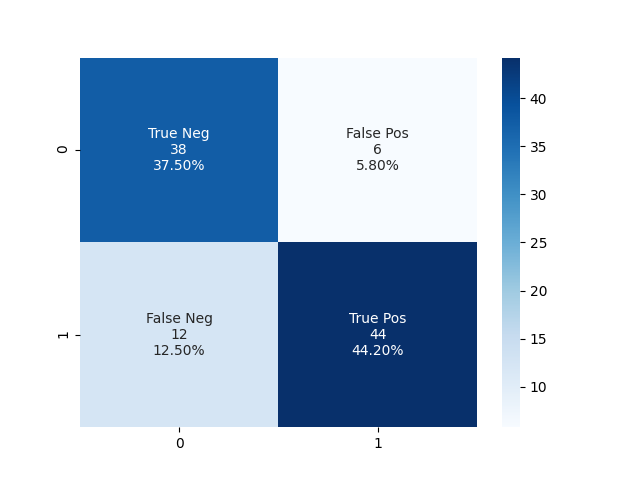
\includegraphics[width=0.49\textwidth,height=0.25\textheight]{./imgs/rf_train.png}}
\subfloat[Confusion Matrix on Testing
set]{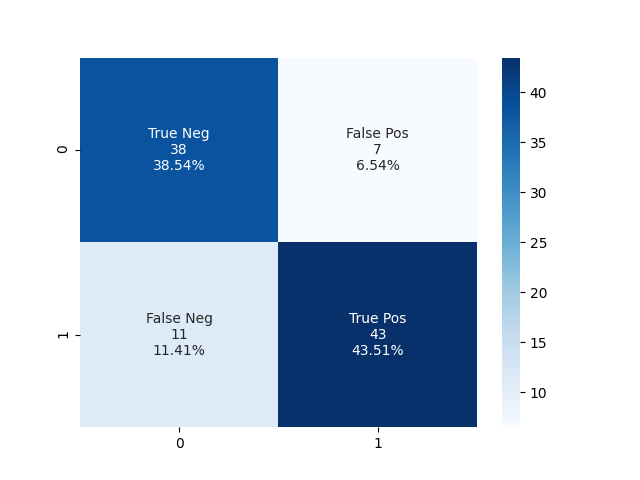
\includegraphics[width=0.49\textwidth,height=0.25\textheight]{./imgs/rf_test.png}}

\caption{Confusion Matrices of RF model evaluated with 5-fold
cross-validation}

\label{fig:rf_cf}

\end{figure}

\hypertarget{xgboost}{%
\subsubsection{XGBoost}\label{xgboost}}

The XGBoost (short for Extreme Gradient Boosting) algorithm is a
variation of the Random Forest concept which utilizes the concept of
gradient boosting to enhance the performance of the model. This
algorithm performs best when being used to model small to medium sized
structured data. The XGBoost algorithm is generally preferred over other
conventional algorithms as it combines many different traits from other
algorithms, such as bagging, gradient boosting, random forest and
decision trees and makes improves upon them through system optimization
and algorithmic enhancements such as regularization, sparsity awareness,
weighted quartile sketch, and so on.

\hypertarget{gradient-boosting}{%
\paragraph{Gradient Boosting}\label{gradient-boosting}}

Gradient boosting is a repetitive algorithm used to leverage the
patterns of mistakes made by a model to strengthen the model using weak
predictions. Basically, the data is modeled very simply and is analyzed
for errors to identify data points that are difficult for the model to
fit. The model is tweaked to fit better for those particular data
points. Finally, this is combined with the original models for an
optimal solution.

The Confusion Matrices plotted from the predictions of the XGB model on
both the training and testing sets are shown in fig.~\ref{fig:xgb_cf}

\begin{figure}
\centering

\subfloat[Confusion Matrix on Training
set]{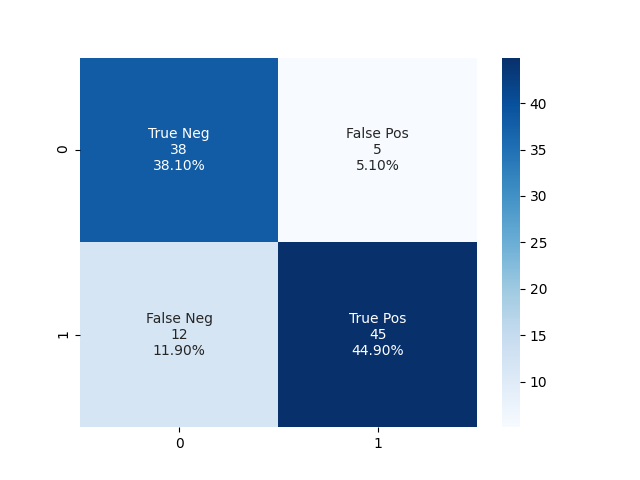
\includegraphics[width=0.49\textwidth,height=0.25\textheight]{./imgs/xbg_train.png}}
\subfloat[Confusion Matrix on Testing
set]{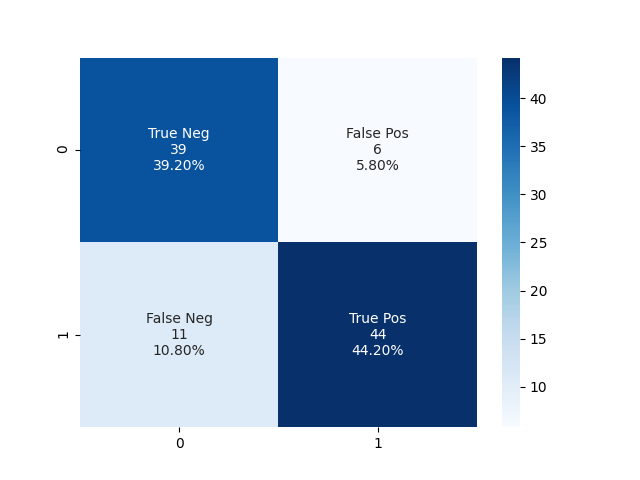
\includegraphics[width=0.49\textwidth,height=0.25\textheight]{./imgs/xbg_test.png}}

\caption{Confusion Matrices of XBG model evaluated with 5-fold
cross-validation}

\label{fig:xgb_cf}

\end{figure}

\hypertarget{results}{%
\section{Results}\label{results}}

The statistics of the final trained models when evaluated on the testing
set are tabulated below in tbl.~\ref{tbl:model_stats}

\hypertarget{tbl:model_stats}{}
\begin{longtable}[]{@{}lll@{}}
\caption{\label{tbl:model_stats}Final statistics of the trained RF and
XGB models evaluated on the testing set}\tabularnewline
\toprule
Attribute & RF & XGB\tabularnewline
\midrule
\endfirsthead
\toprule
Attribute & RF & XGB\tabularnewline
\midrule
\endhead
Accuracy & 0.8199 & 0.8339\tabularnewline
95\% CI & (0.8017, 0.8371) & (0.8162, 0.8505)\tabularnewline
No Information Rate & 0.5 & 0.5\tabularnewline
P-Value {[}Acc \textgreater{} NIR & \textless{} 2.2e-16 & \textless{}
2.2e-16\tabularnewline
Kappa & 0.6399 & 0.6677\tabularnewline
Mcnemar's Test P-Value & 6.889e-07 & 1.277e-07\tabularnewline
Sensitivity & 0.7706 & 0.7835\tabularnewline
Specificity & 0.8692 & 0.8842\tabularnewline
Pos Pred Value & 0.8549 & 0.8713\tabularnewline
Neg Pred Value & 0.7912 & 0.8033\tabularnewline
Prevalence & 0.5000 & 0.5000\tabularnewline
Detection Rate & 0.3853 & 0.3917\tabularnewline
Detection Prevalence & 0.4507 & 0.4496\tabularnewline
Balanced Accuracy & 0.8199 & 0.8339\tabularnewline
`Positive' Class & no & no\tabularnewline
\bottomrule
\end{longtable}

The \emph{Accuracy} and \emph{Kappa} values of both models are very
similar, indicating that both models perform very similarly for this
particular dataset. Both models perform consistently over the testing
set with regards to their performance on the training set and are able
to classify the datapoints. However, the XGB model has an accuracy of
83.39\% which is slightly higher than that of the RF model, which is
approximately 82\%. The XBG model also clearly outperforms the RF model
in almost every other aspect, which was as expected.

Both models assign an `Feature Importance' score to each attribute,
which is calculated by the amount that the particular attribute's split
point improves the performance measure, weighed by then number of
observations the node is responsible for. In our case, the performance
measure is the \emph{Gini Index}, which is used to select the splits
points. The plots of the 20 most important attributes according to the
RF model and the XGB model can be seen in fig.~\ref{fig:rf_imp} and
fig.~\ref{fig:xgb_imp} respectively.

\begin{figure}
\centering

\subfloat[Feature importance plot from RF
model]{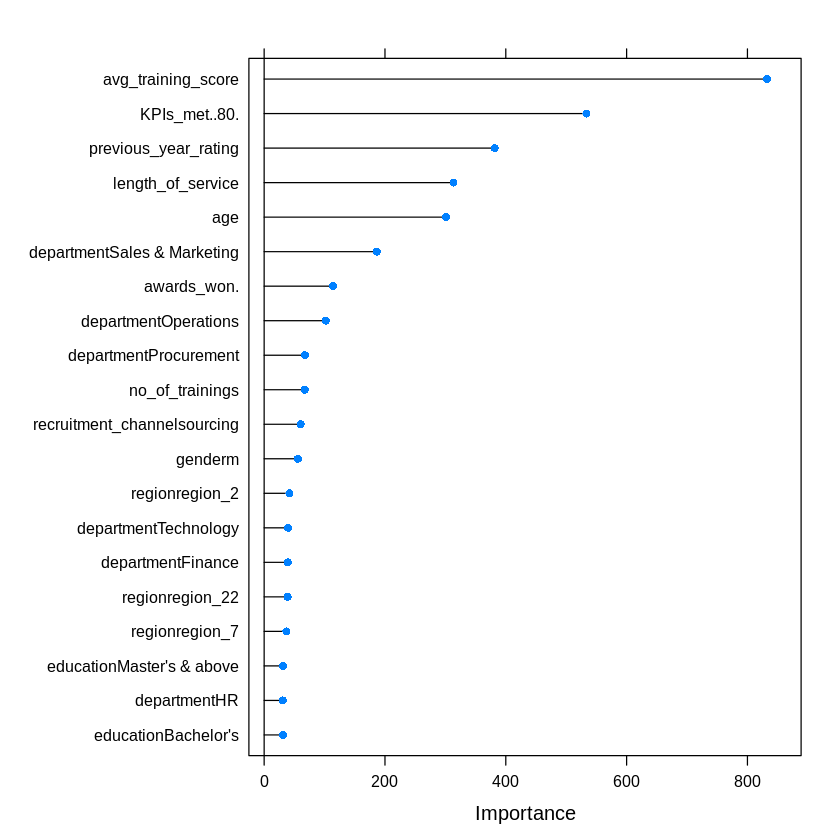
\includegraphics[width=\textwidth,height=0.49\textheight]{./imgs/rf_feat_imp.png}\label{fig:rf_imp}}\\
\subfloat[Feature Importance plot from XGB
model]{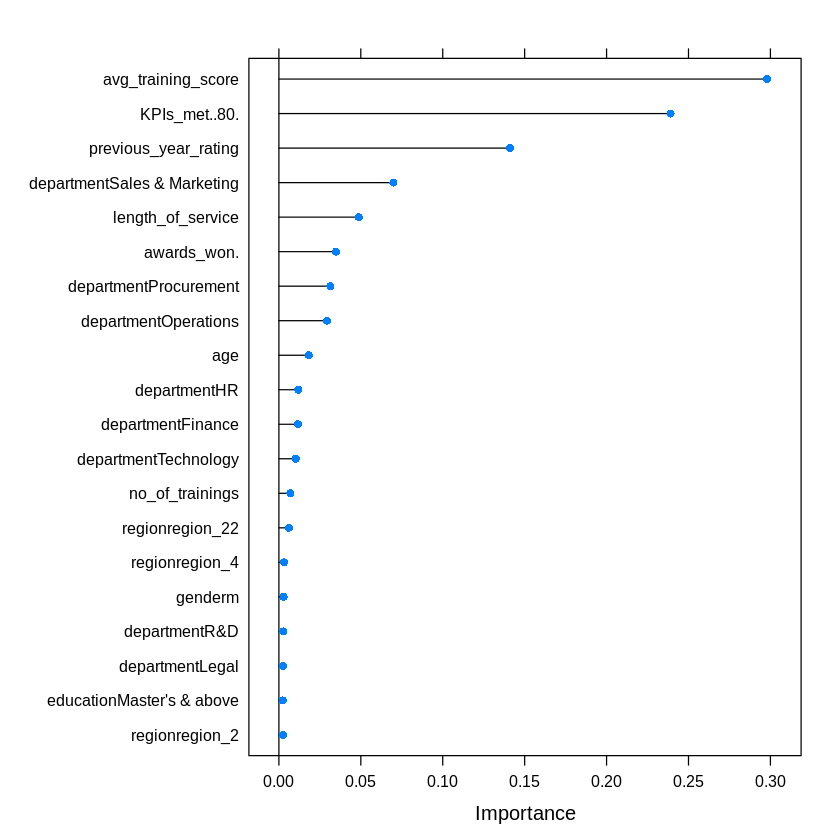
\includegraphics[width=\textwidth,height=0.49\textheight]{./imgs/xb_feat_imp.png}\label{fig:xgb_imp}}

\caption{20 most important features as scored by the RF and XGB models}

\label{fig:imp_feats}

\end{figure}

\newpage

We notice that the list of the 10 most important features according to
both the Random Forest and XGBoost models are nearly identical with the
exception of no\_of\_trainings and departmentHR. This tells us that the
other attributes can be discarded to get improved performance from the
models.

\hypertarget{conclusion}{%
\section{Conclusion}\label{conclusion}}

In this paper, we have demonstrated the use of the Random Forest and
XGBoost machine learning algorithms in predicting an employee's
promotion status. We also used the trained models to determine which
attributes have the most impact on said promotion status. Through this,
we can see the use of machine learning as a predictive decision making
tool or at least a suggestive tool is a fully viable solution for the
presented problem. With fairly limited data and computational resources,
we were able to train algorithms to perform with significantly good
accuracy.

In the future, higher accuracy and more efficient models can be achieved
with higher volumes of data and more careful tuning of the models'
parameters. We can also improve the models' accuracy by retraining the
models on just n-most important features as seen from
fig.~\ref{fig:imp_feats}. Furthermore, we can expand this research by
applying various other machine learning approaches, such as Support
Vector Machines and Recurrent Neural Networks.

\begin{thebibliography}{8}
\bibitem{ref-Quddus2019}{}%
{Abdul, Q., Mohammed, A.: HR ANALYTICS: A MODERN TOOL IN
HR FOR PREDICTIVE DECISION MAKING. Journal of Management. 6, 51--63
(2019).}

\bibitem{ref-Breiman2001}{}%
{Breiman, L.: Random forests. Machine Learning. 45, 5--32
(2001).}

\bibitem{ref-ChenG16}{}%
{Chen, T., Guestrin, C.: XGBoost: {A} scalable tree
boosting system. CoRR. abs/1603.02754, (2016).}

\bibitem{ref-Marler2017}{}%
{Marler, J.H., Boudreau, J.W.: An evidence-based review
of HR analytics. The International Journal of Human Resource Management.
28, 3--26 (2017).}

\bibitem{ref-Jin2020}{}%
{Jin, Z., Shang, J., Zhu, Q., Ling, C., Xie, W., Qiang,
B.: RFRSF: Employee turnover prediction based on random forests and
survival analysis. In: Huang, Z., Beek, W., Wang, H., Zhou, R., and
Zhang, Y. (eds.) Web information systems engineering -- WISE 2020. pp.
503--515. Springer International Publishing, Cham (2020).}

\bibitem{ref-Liu2019}{}%
{Liu, J., Wang, T., Li, J., Huang, J., Yao, F., He, R.: A
data-driven analysis of employee promotion: The role of the position of
organization. 2019 IEEE international conference on systems,man and
cybernetics (SMC). pp. 4056--4062 (2019).}

\end{thebibliography}

\end{document}
